\subsection{Определения}

Пусть дан массив из $n$ элементов. \\
\textbf{Дерево отрезков} - это двоичное дерево, в котором:

\begin{itemize}
    \item Есть $n$ листьев, соответствующих отрезкам единичной длины
    \item Есть вершины с двумя сыновьями. Правый сын соответствует отрезку,
    следующему сразу за отрезком левого сына. Вершина соответствует
    объединению отрезков сыновей
    \item Корень дерева соответствует всему массиву (отрезку $[1; n]$).
\end{itemize}

\textbf{Запрос сверху} на отрезке $[L, R]$ начинается в корне.
Если сейчас рассматривается вершина, отрезок которой не лежит полностью в
отрезке $[L, R]$, то запрос рекурсивно вызывается от тех сыновей, отрезки которых
пересекаются с $[L, R]$. Иначе рекурсивных вызовов от сыновей не происходит.
В обоих случаях вершина считается посещенной и в ней выполняются какие-то
действия, специфичные для запроса.

Пример запроса сверху указан на рисунке \ref{fig:segtree_example}. Здесь дерево отрезков на пяти элементах и запрос на отрезке $[2;4]$. Будет посещено пять выделенных вершин.

\begin{figure}[hbt!]
    \centering
    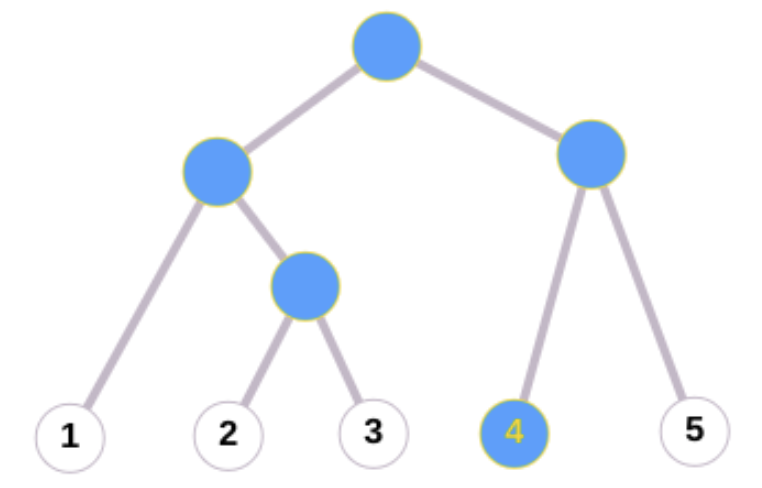
\includegraphics[scale=0.28]{images/segtree_example.png}
    \caption{Пример запроса к дереву отрезков}
    \label{fig:segtree_example}
\end{figure}

\subsection{Постановка задачи}

\textbf{Дано:} Распределение вероятностей на запросах-отрезках границами из $[1; n]$

\textbf{Необходимо:} построить дерево отрезков, для которого минимально среднее
количество посещенных вершин при запросах сверху.

Интересует как точное решение за как можно более лучшую асимптотику, так и
приближенное за сложность нахождения $O(n + S)$ или $O(n + S \log S)$, где $S$ -
количество отрезков с ненулевой вероятностью

\subsection{Мотивация}

Дерево отрезков - это мощная структура данных, которая позволяет решать большое количество задач. 
Если дан массив $a$ из $n$ элементов, то она позволяет эффективно:

\begin{itemize}
    \item Отвечать на запросы $f(a_L, f(\dots, a_R)\dots)$, где $f$ - произвольная ассоциативная функция с двумя аргументами
    \item Изменять элементы $a_L,\dots,a_R$ для некоторых типов изменений
\end{itemize}

Пример: запросы суммы/минимума на подотрезке массива и прибавления числа ко всем элементам подотрезка массива.

Обычно для этого в каждой вершине дерева отрезков хранится значение функции на соответствующем подотрезке массива и информация о том, нужно ли применить какие-то отложенные изменения к сыновьям данной вершины.

Запросы на расчёт функции находятся с помощью запроса сверху и объединения результатов для посещенных вершин. Запросы на изменение тоже совершаются с помощью запросов сверху, для посещенных вершин происходит изменение информации в них нужным образом.

Если для каждой вершины дерева с двумя сыновьями её отрезок разбивается примерно пополам и каждой половине соответствуют её сыновья, то можно показать, что при запросе сверху посещается $O(\log n)$ вершин.

При этом большое количество задач различных тематик можно свести к запросам на подотрезках массива. Примеры таких задач:

\begin{itemize}
    \item Для дерева из $n$ вершин после препроцессинга за $O(n)$ можно отвечать на запросы минимального общего предка за $O(\log n)$
    \item Для строки из $n$ символов после построения суффиксного массива и дополнительного препроцессинга за $O(n)$ можно находить длину наибольшего общего префикса двух любых её подстрок
    \item Если нам дано $n$ прямоугольников на плоскости со сторонами, параллельными осям координат, то можно найти площадь их объединения за $O(n \log n)$
\end{itemize}

Как уже было сказано, если для каждой вершины разбивать её подотрезок на две равные части, то сложность запроса к дереву отрезков $O(\log n)$. Но нам может быть известно распределение вероятностей запросов, и в таком случае можно построить более оптимальное дерево. Таким образом решение задачи, поставленной в дипломе, может привести к ускорению на большом классе задач и может представлять не только теоретический, но и практический интерес.

Кроме того надо заметить, что данный диплом далеко не первый, посвященный вопросу построения оптимальных структур данных при известном распределении вероятностей запросов. В частности, смежная задача построения статически оптимального дерева поиска хорошо изучена, её результаты будут использоваться в дальнейшем.